\documentclass[12pt]{article}

\title{Using Catmull-Rom curves to visualize the complex Mandelbrot trajectories}
\author{S. Halayka\footnote{sjhalayka@gmail.com}}
\date{\today}

\usepackage{listings}
\usepackage{cite}
\usepackage{xcolor}
\usepackage{graphicx}
\usepackage{setspace}
\usepackage{amsmath}
\usepackage{url}

\usepackage{caption}
\usepackage{subcaption}

%\usepackage[margin=1in]{geometry}
%\doublespace
\begin{document}




\maketitle

\begin{abstract}
The trajectories of the Mandelbrot set are visualized using Catmull-Rom curves and OpenGL.
\end{abstract}



\section{Introduction}

As discussed in many papers, a 2D scalar field of complex magnitudes (e.g. $|Z| = \sqrt{Z_x^2 + Z_y^2}$) results from calculating the complex Mandelbrot set when using a finite 2D lattice of regularly spaced vertices as input.

Iteration is performed to obtain the trajectories of a complex Mandelbrot set.
The criterion for an input location being in the set is that the location's trajectory's end vertex magnitude is always less than some threshold.
For this paper, we use a maximum iteration count of $500$, and a threshold value of $4.0$.
Once all of the Mandelbrot set's trajectories have been generated, they are converted to Catmull-Rom curves, to be visualized using OpenGL. 

The primary motivation for the exploration of the trajectories of the complex Mandelrbrot set was to introduce a new type of visualization.


\section{Why Catmull-Rom curves?}

Catmull-Rom curves seem to encode a higher degree of fidelity, when it comes to the line passing through all of the control points.
This is unlike B\'ezier curves, where the line is only guaranteed to go through the beginning and end control points.

Catmull-Rom curves offer $C_1$ continuity -- continuity in both position and tangent vectors.
As such, the closed (periodic) loops of the Mandelbrot set are easy to visualize.

Catmull-Rom curves are as computationally intensive as B\'ezier curves, but not much more.

Catmull-Rom curves are pretty.












\begin{thebibliography}{9}
\bibitem{bourke} Bourke. (2018) ``3D volumetric fractal trajectories''
\bibitem{halayka2} Halayka. (2018) ``Visualizing the escape paths of quaternion fractals''
\end{thebibliography}



\pagebreak




\begin{figure} 
\centering
  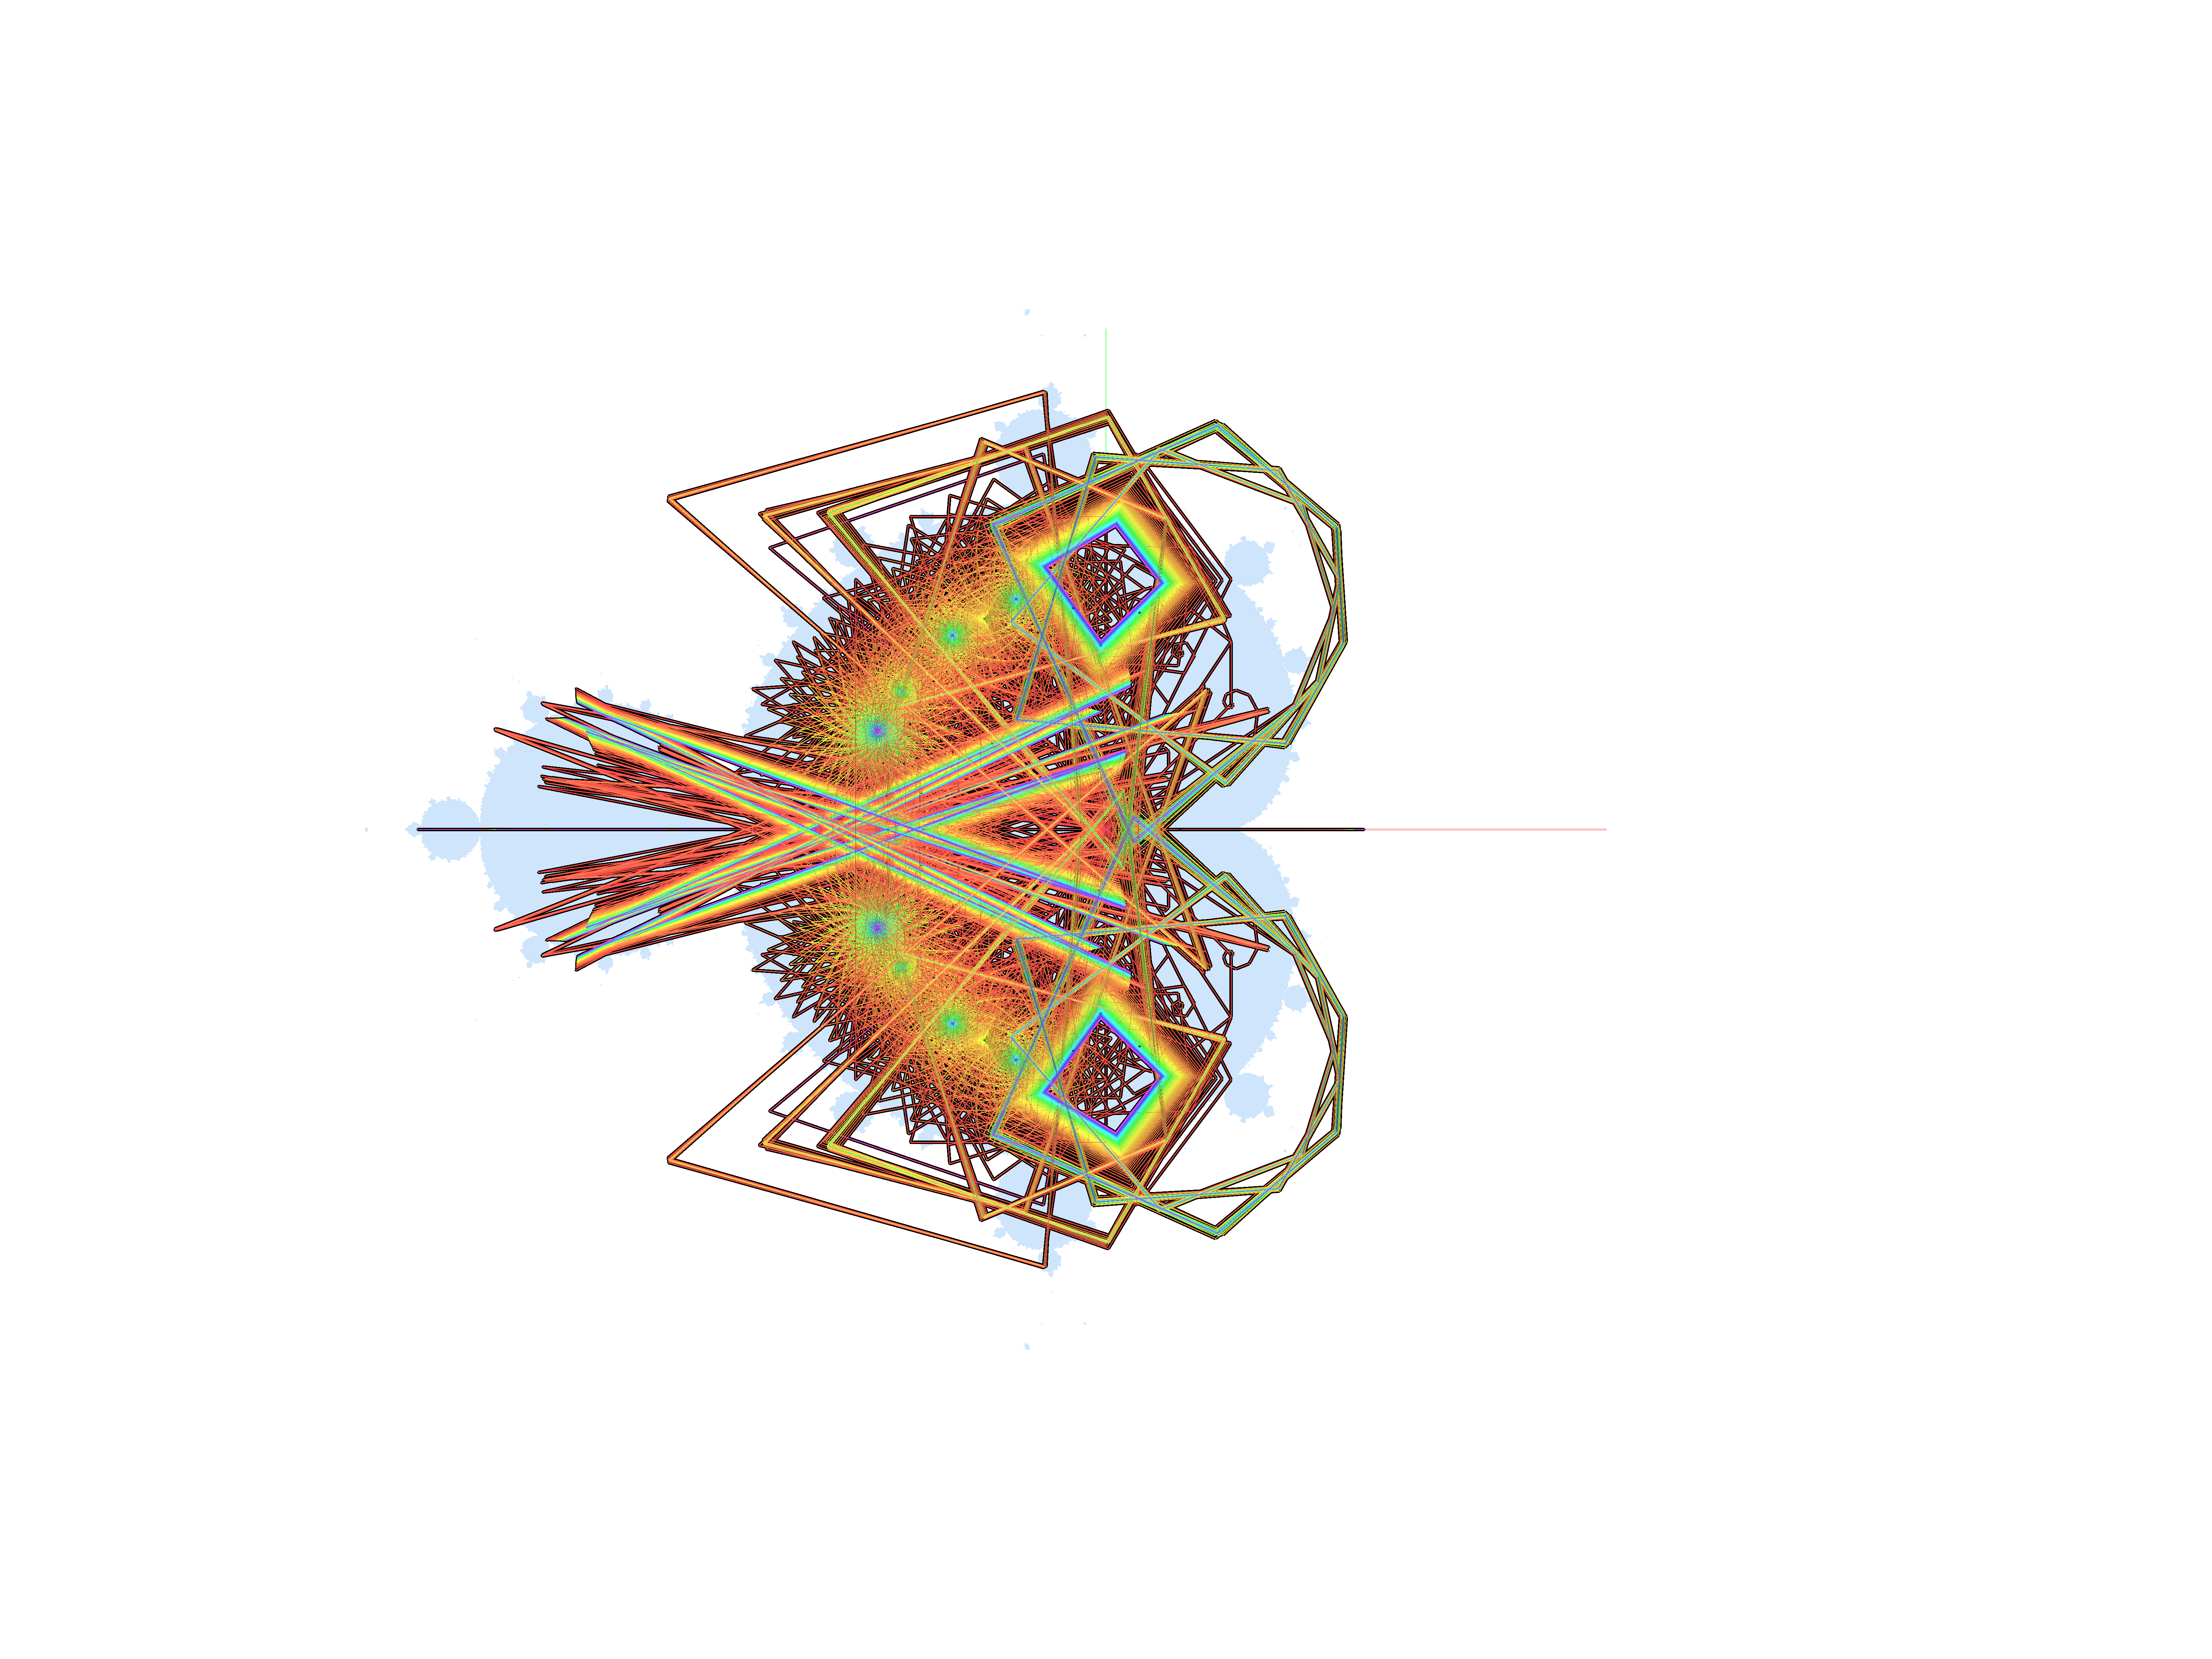
\includegraphics[width = 4 in]{rainbow_500_iterations_non_curved.png}	
  \caption{Iterations = 500. Actual trajectories are drawn.}
\end{figure}

\begin{figure} 
\centering
  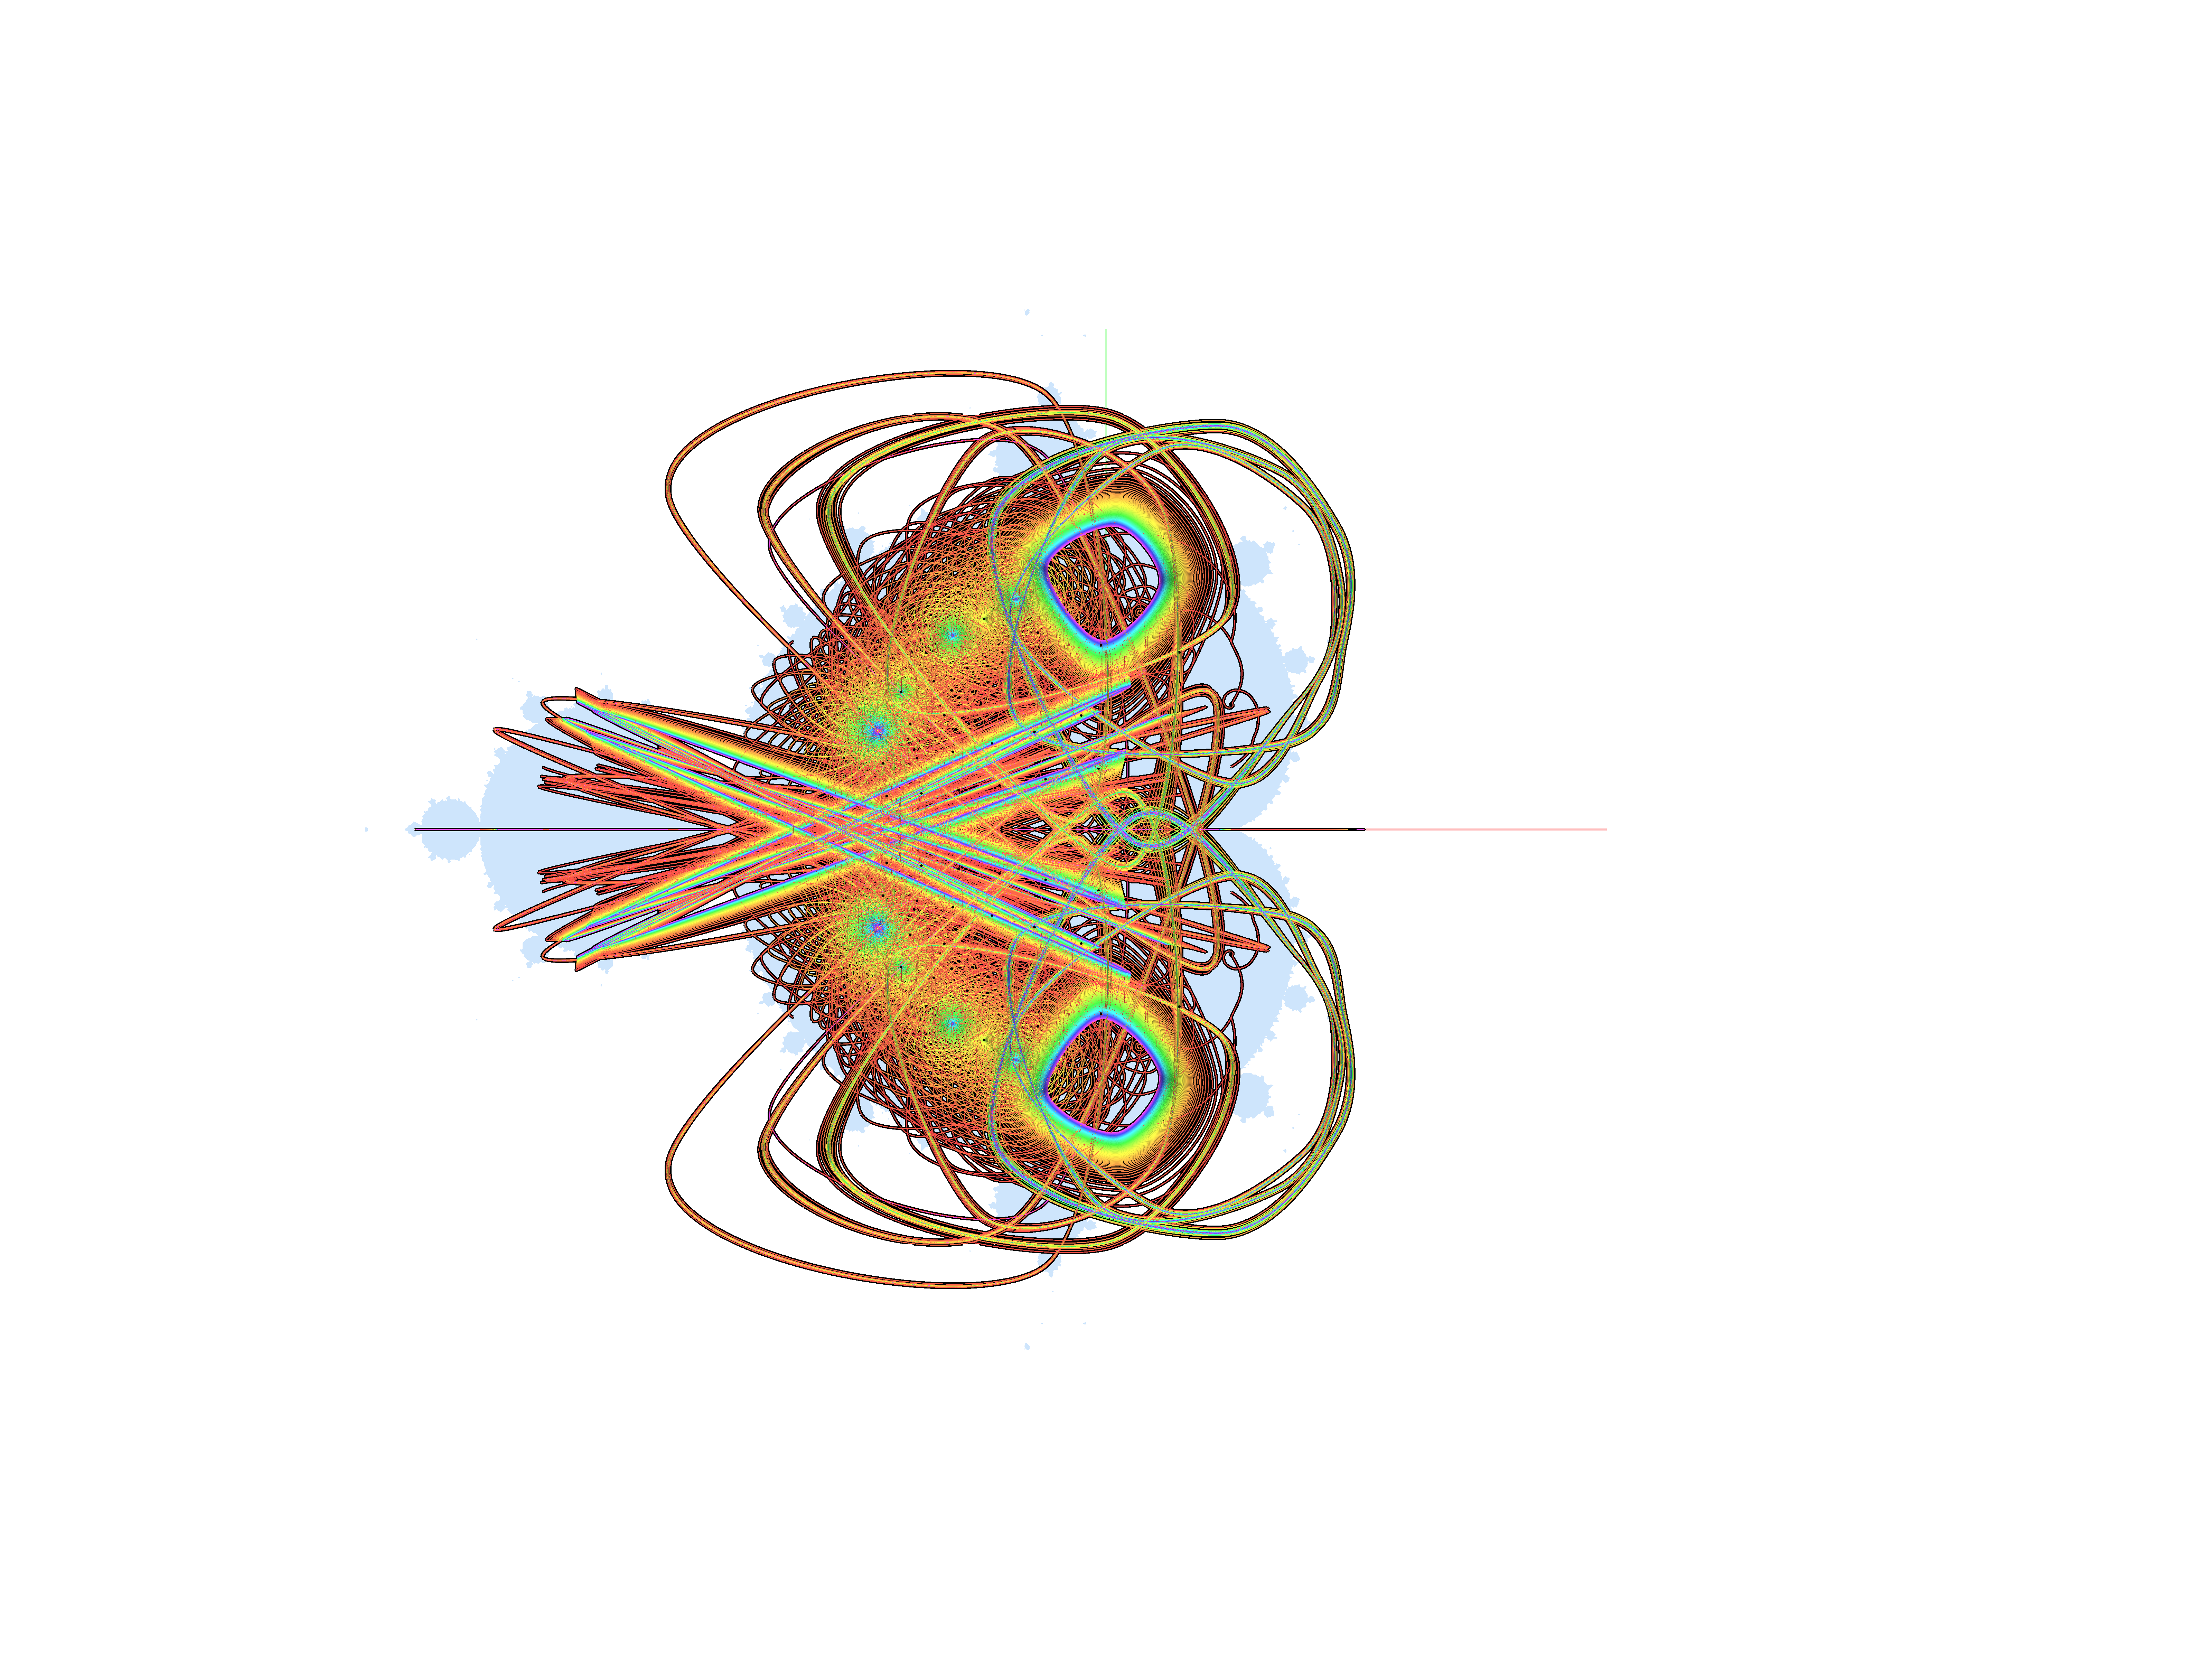
\includegraphics[width = 4 in]{rainbow_500_iterations.png}	
  \caption{Iterations = 500. Catmull-Rom trajectories are drawn.}
\end{figure}

\begin{figure} 
\centering
  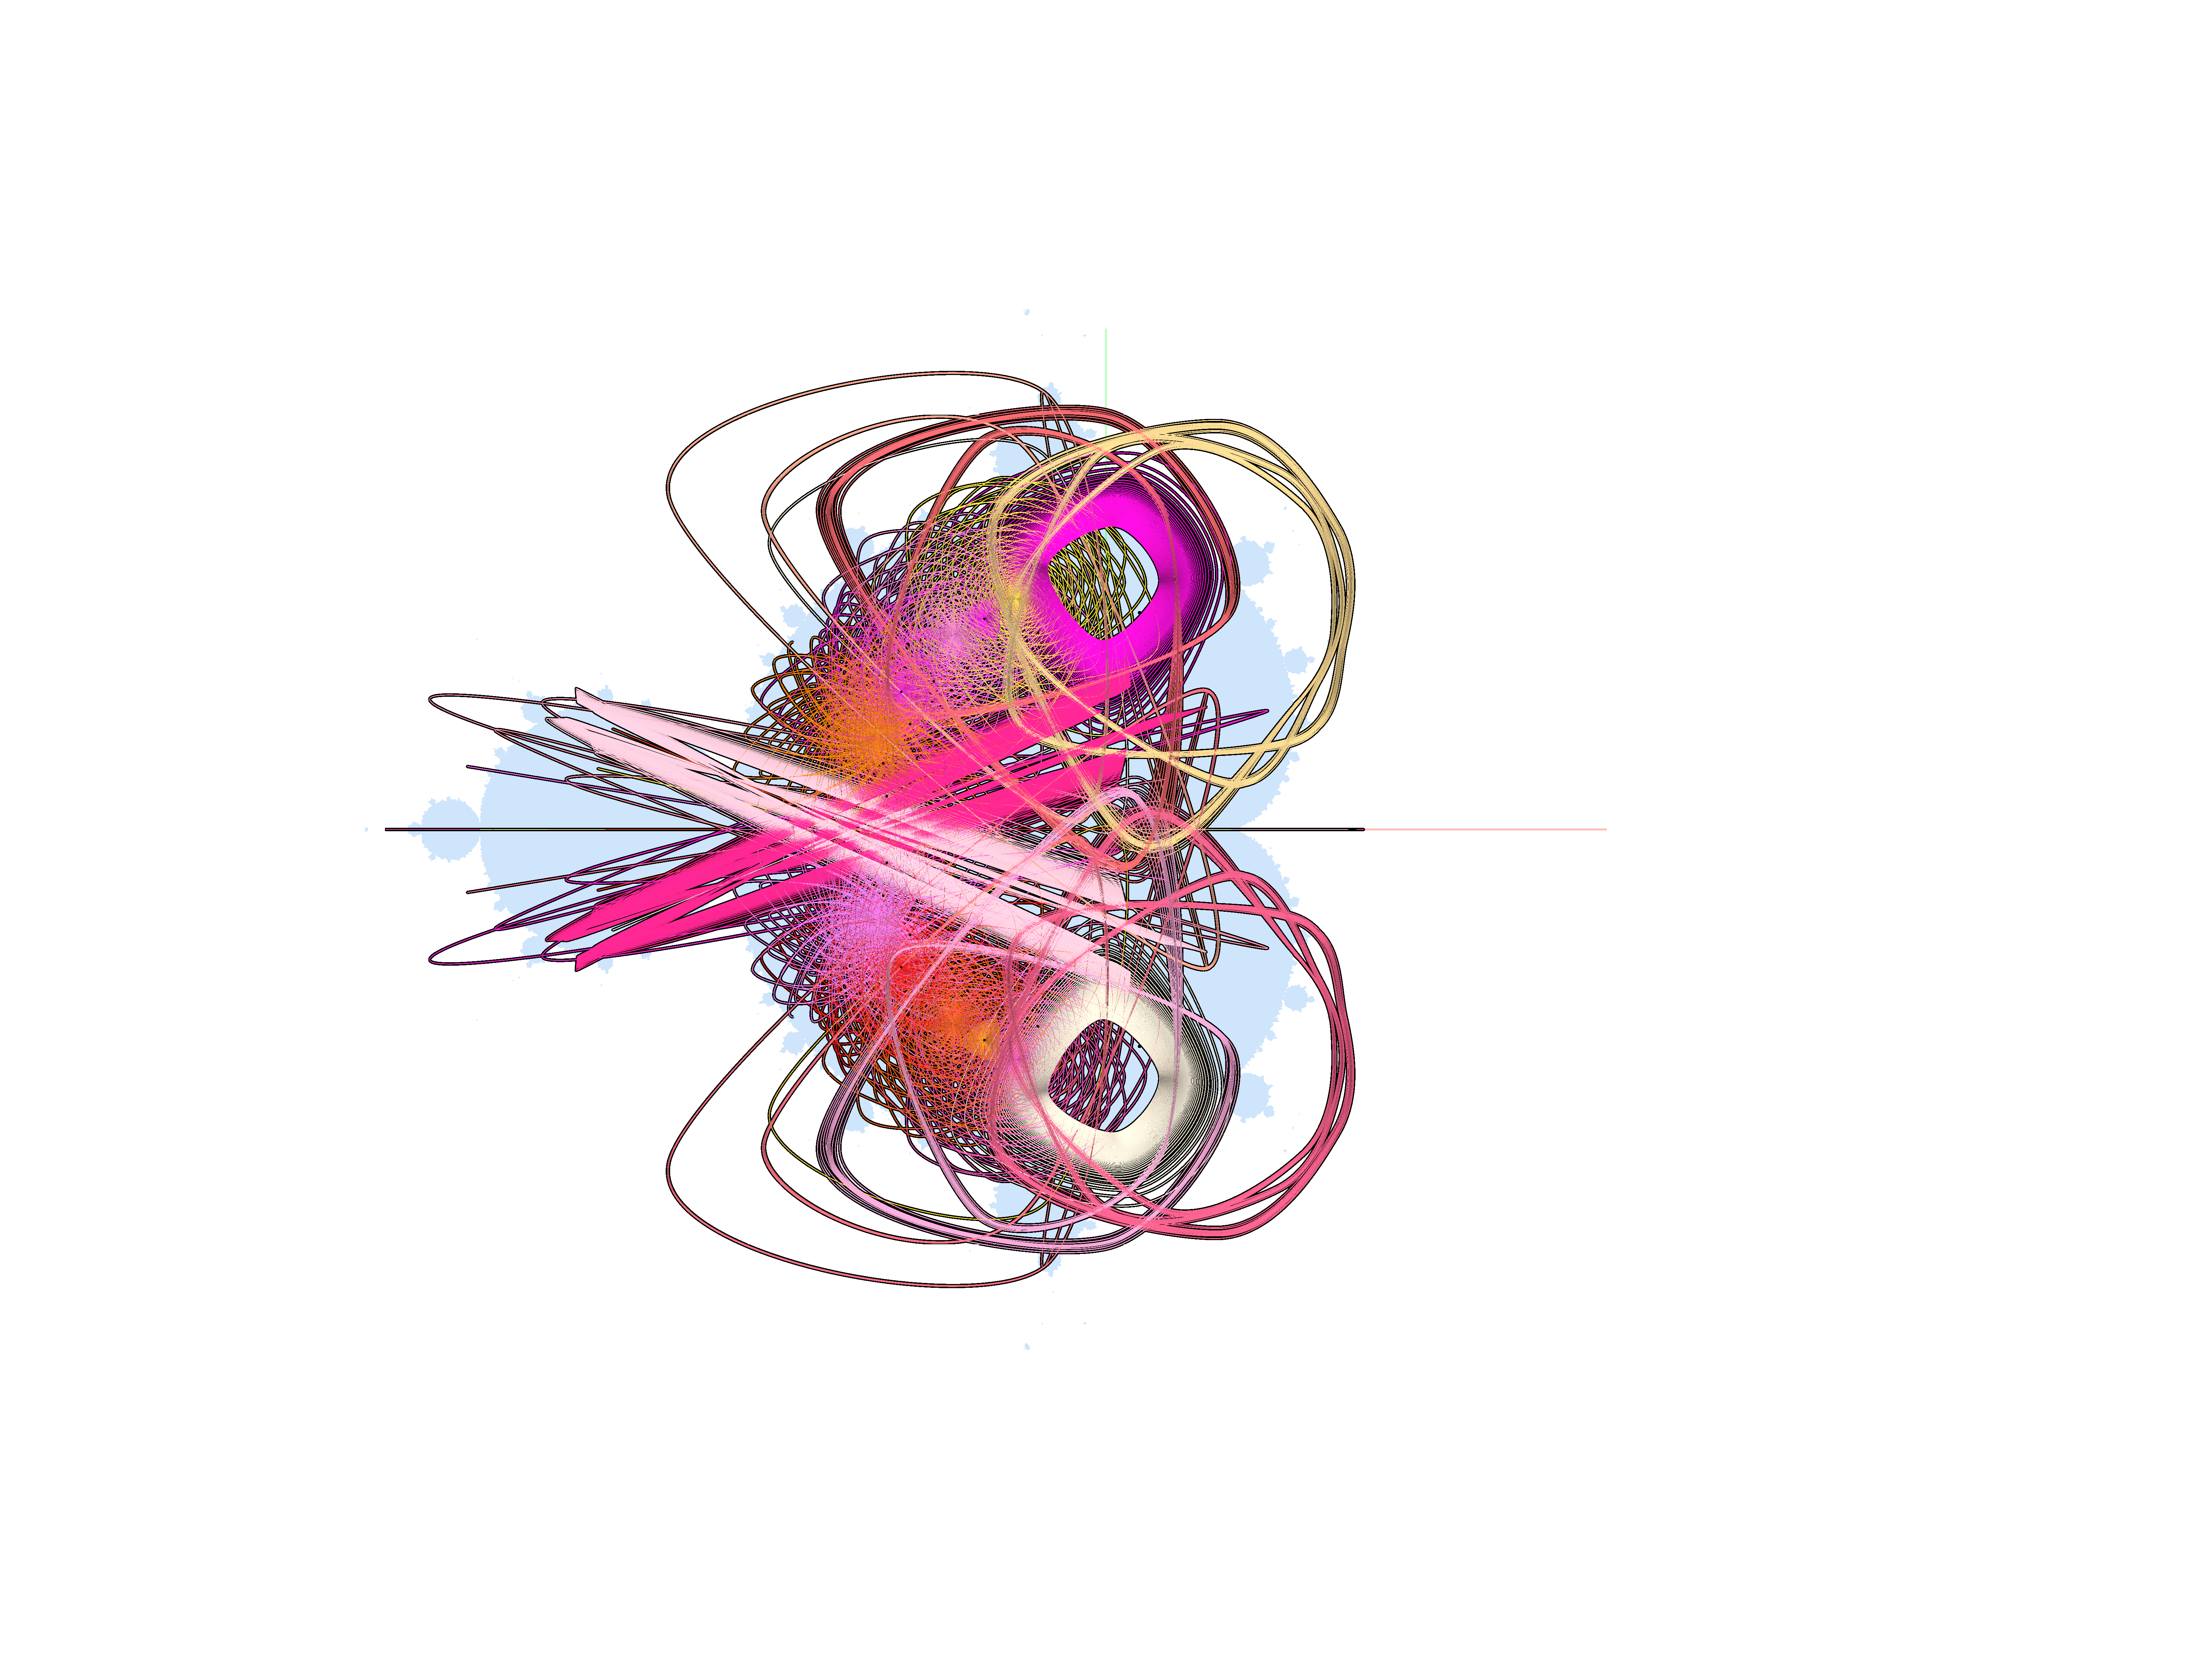
\includegraphics[width = 4 in]{pseudorandom_500_iterations.png}	
  \caption{
Iterations = 500. 
Catmull-Rom trajectories are drawn.
Pseudorandomly-assigned colours are used, to help differentiate between the individual orbits.}
\end{figure}

\end{document}









